The statecharts in this section provide an overview of the communications and states of the individual components of the game. In the class level statecharts, the communication within the separate classes are given. In the system level statechart, the communication between the individual components is shown. The communication consists of messages exchanged between classes; these messages correspond to the messages and signals shown in the MSCs. \\
The following syntax is used for transitions in the statecharts: trigger [condition] / triggered. Here, 'trigger' denotes the event that triggers the transition; 'condition' specifies under what conditions the transition can be taken and 'triggered' denotes the events that are triggered because of the transition. If transitions with similar 'trigger' events occur, they are listed as separate transitions. In a condition with several constraints, each constraint is separated by a '\&'. If multiple 'triggered' events are possible, they are separated by a ';' and listed in the order in which they are triggered. For example, in the Board statechart, the getValidTiles()-transition between the states 'Controller Initialized' and 'NOP' triggers both the events getValidTiles() en notifyViewer(). As shown in the MSCs for tiles exchange, first getValidTiles() is called and thereafter notifyViewer().

\subsection{Class level}

    \subsubsection{Board}
	First the board is initialized, then the board has to preinitialize the controller. After that the board initializes the robots and sends a postinitialize message to the controller. Then the board goes to the NOP state from which it can answer requests from robots and the controller. \\
\\
Whenever a robot requests an invalid move via the moveRequest() function, the board sends out a moveRequest() == FAILED message and returns to the NOP state. But when a robot requests a correct move, the new position is calculated and stored using the functions calcuateNewLocation() and saveLocation(). \\
\\
Normally the board now goes to the RequestedRobotMoved state from which it will send a hint if the robot stept on a hinttile, the board will always notify the controller that the board has been updated via the Controller.notifyViewer() function.\\
\\
If the requested move would mean that other robots will get moved the board goes to the RequestedRobotMoved state with the Controller.notifyAutoMovement() function which means that the other robot will receive a notifyAutoMovement to let him know that he has been moved, all the other functions called are the same as with the regular move.\\
\\
When a robot moves to it's homeTile, the boardResponse will be WIN and the game ends, then the board goes to the Game Over state and it can terminate or start a new game, note the choice between termination or new game is nondeterministic.\\
\\
Every time a robot has made a move, the controller requests a tile-exchange via the requestTilesExchange() function, this exchange is performed by the board.\\
	
	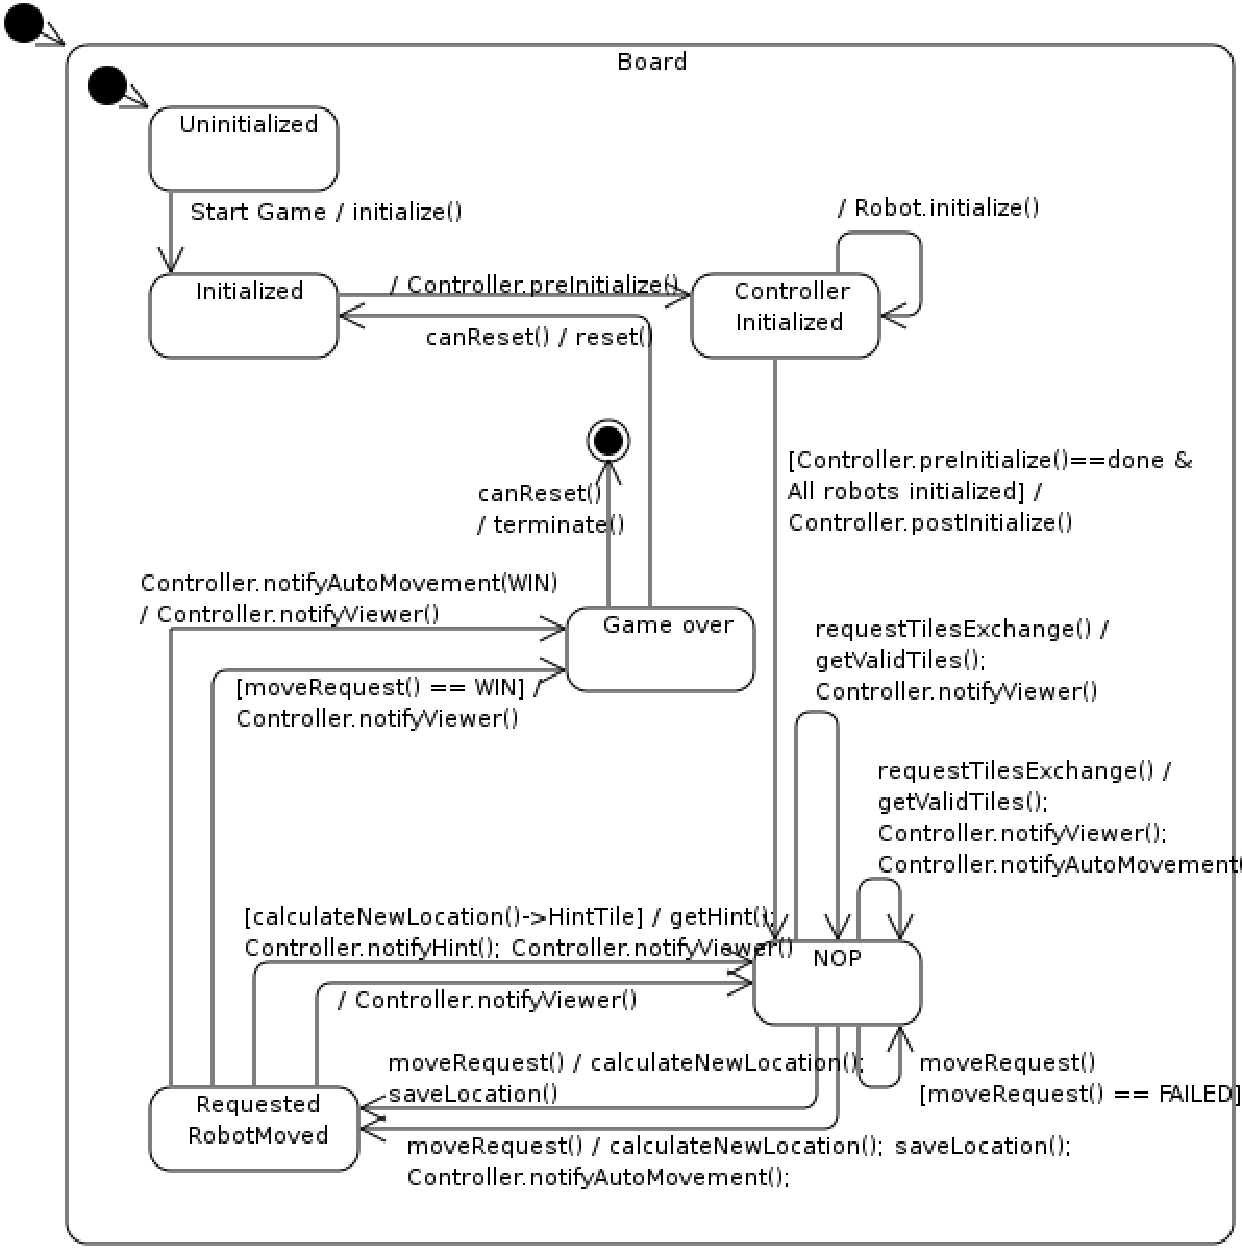
\includegraphics[width=\linewidth]{statecharts/board.pdf}

	\subsubsection{Controller}
	The controller initializes in two phases, the first phase is the preInitialize() during which it waits for other classes to initialize. The second phase is the postInitialize() function, when the controller calls this function, it knows that all the other classes have been initialized and is aware of the state of all the classes and goes to the NOP state from which most actions take place. After initializing the controller goes to the NOP state from which everything happens\\
\\
If a robot requests a move, the board answers the moveRequest and the controller goes in to the MoveRequestedProcessed state. After that it goes to a new state depending on the response of the board. If the move is declined the controller goes back to the NOP state, the robot is not moved. If the robot is allowed to do it's move the controller switches 2 tiles using Board.requestTilesExchange() and sends a Robot.notifyHint() if needed, it will go to the TilesExchangeProcessed state. If this move also made other robots move, those other robots will receive a notifyAutoMovement from the controller. If the robot landed on it's hometile the controller will send a notifyGameOver() to let the viewer know that the game has ended, it will also send a terminate() function to the robot and a reset() function to the board, after that the controller will terminate itself.\\
\\
After the 2 tiles are switched the robots that have been moved by this tileswitch are notified via the Robot.notifyAutoMovement().\\
\\
After every successful move and tile exchange the controller also calls the Viewer.notifyStateChange() function to let the viewer know the board has been changed.\\
	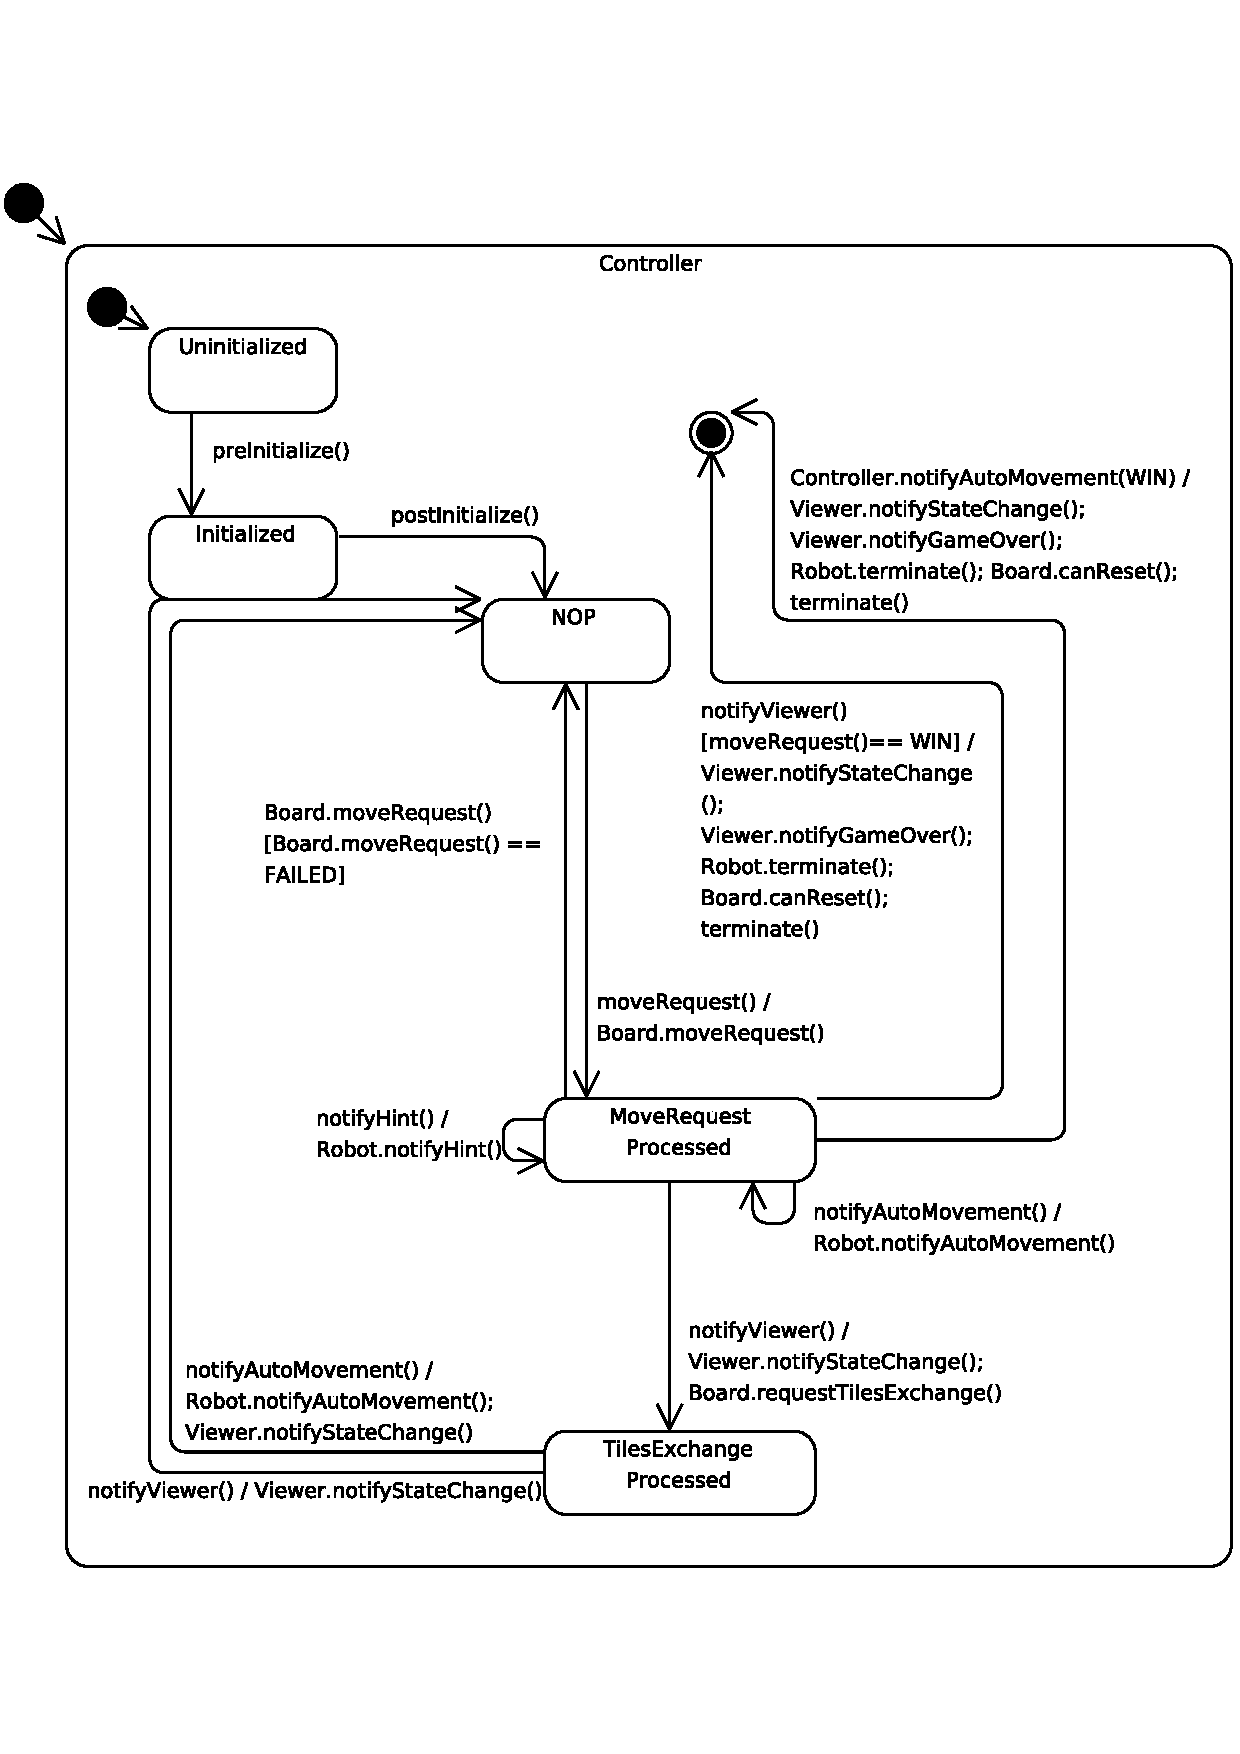
\includegraphics[width=\linewidth]{statecharts/controller.pdf}

	\subsubsection{Viewer}
	After being initialized the viewer comes in the NOP state, in this NOP state the viewer will receive updates from the board and makes sure these are shown via the updateView() function.\\
\\
At the end of the game the viewer is terminated.\\
	
	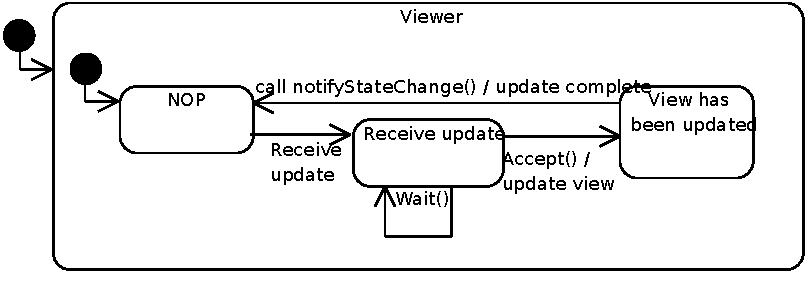
\includegraphics[width=\linewidth]{statecharts/view.pdf}

	\subsubsection{Robot}
	The robot class gets initialized by the controller, it starts at a randomly picked spot, which can be a normal tile, a hint tile or a conveyer tile. Depending on the tile the robot goes to the OnHintTile state or the OnRegularOrConveyorTile state.\\
\\
In each of these states the robot can receive a notifyAutomovement() if it get's moved, if this occurs the robot does remain in the same state. It can also receive a terminate() function, which means that another robot has won and this robot has lost and must therefor terminate.\\
\\
If a robot requests a move it goes to the MoveRequestFromHintTile or the MoveRequestedFromRegularOrConveyorTile state depending on the current tile. When the robot is in this MoveRequested, the controller can give back 3 responses: WIN, SUCCES and FAILURE.\\
\\
If the response equals WIN, the robot has reached it's hometile and has won the game, it will go to the OnHomeTile state and then terminate. \\
\\
If the response equals SUCCES the request move is allowed and the robot is moved, if the robot has stepped on a hintTile it will receive a hint via the notifyHint() function and go to the OnHintTile state, if the robot has reached a regularTile or a conveyorTile it goes to the OnRegularOrConveyorTile and receive a notifyAutoMovement() function if it has been moved by a conveyorTile.\\
\\
If the resoponse equals FAILED the robot will stay at it's current tile and nothing special will happen.\\
	
	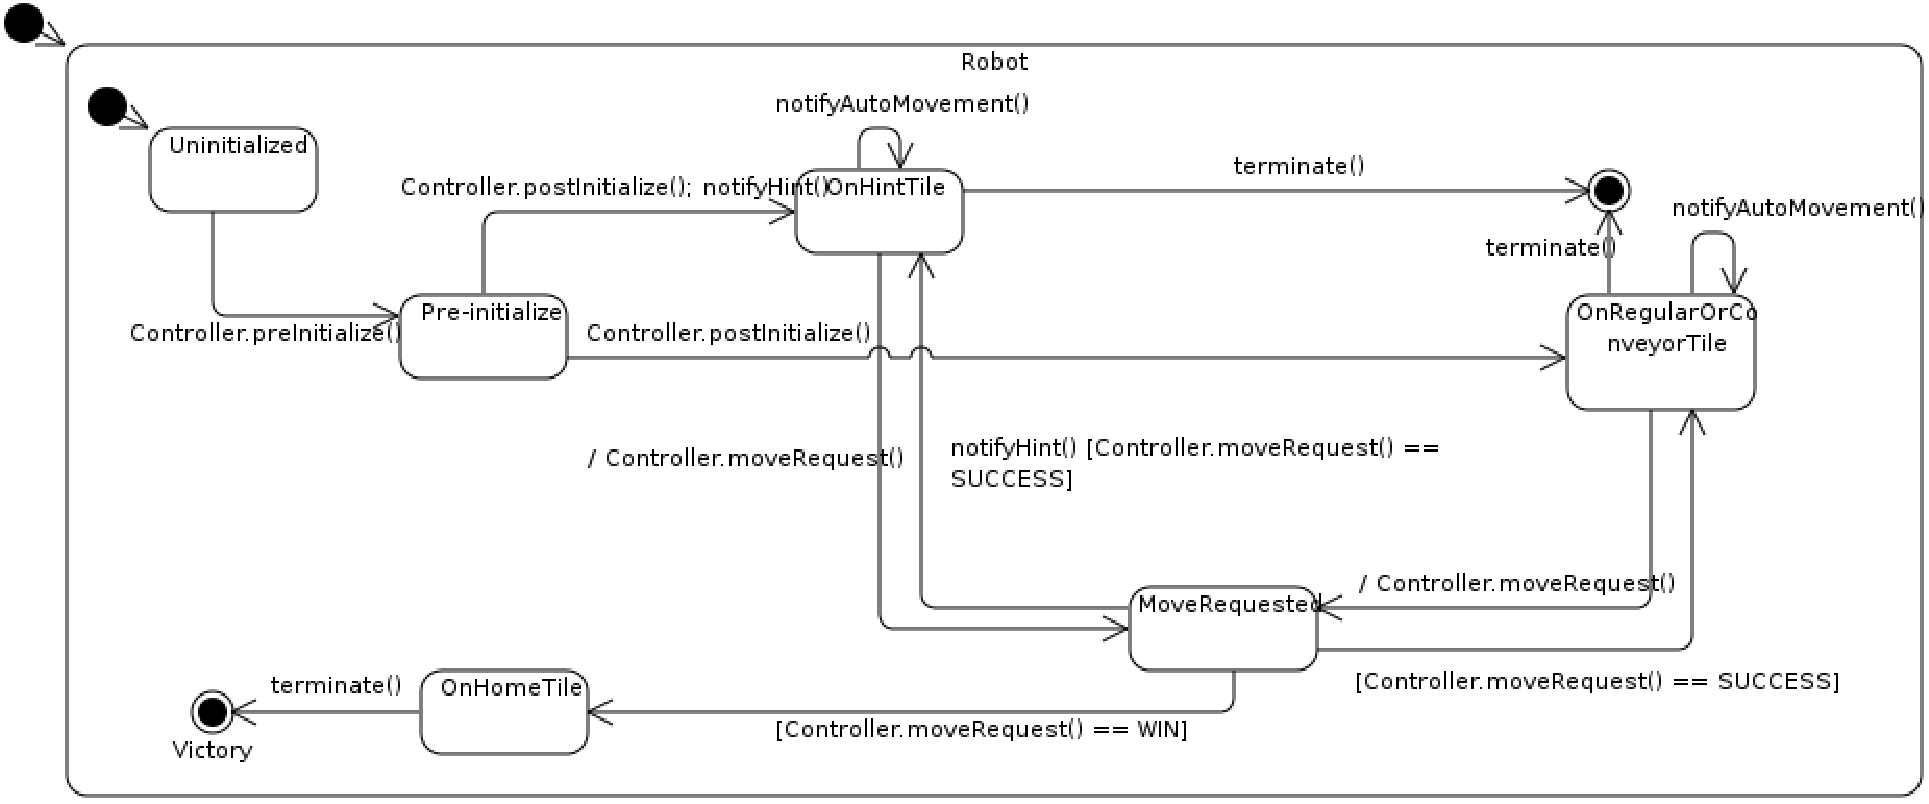
\includegraphics[width=\linewidth]{statecharts/robot.pdf}

\subsection{System level}
	The following graph is our system level state chart, which contains all our class level state charts and gives an overview of the complete system. Although this state chart is mostly trivial, it gives a more complete view of the entire system, thus it is shown below.\\

	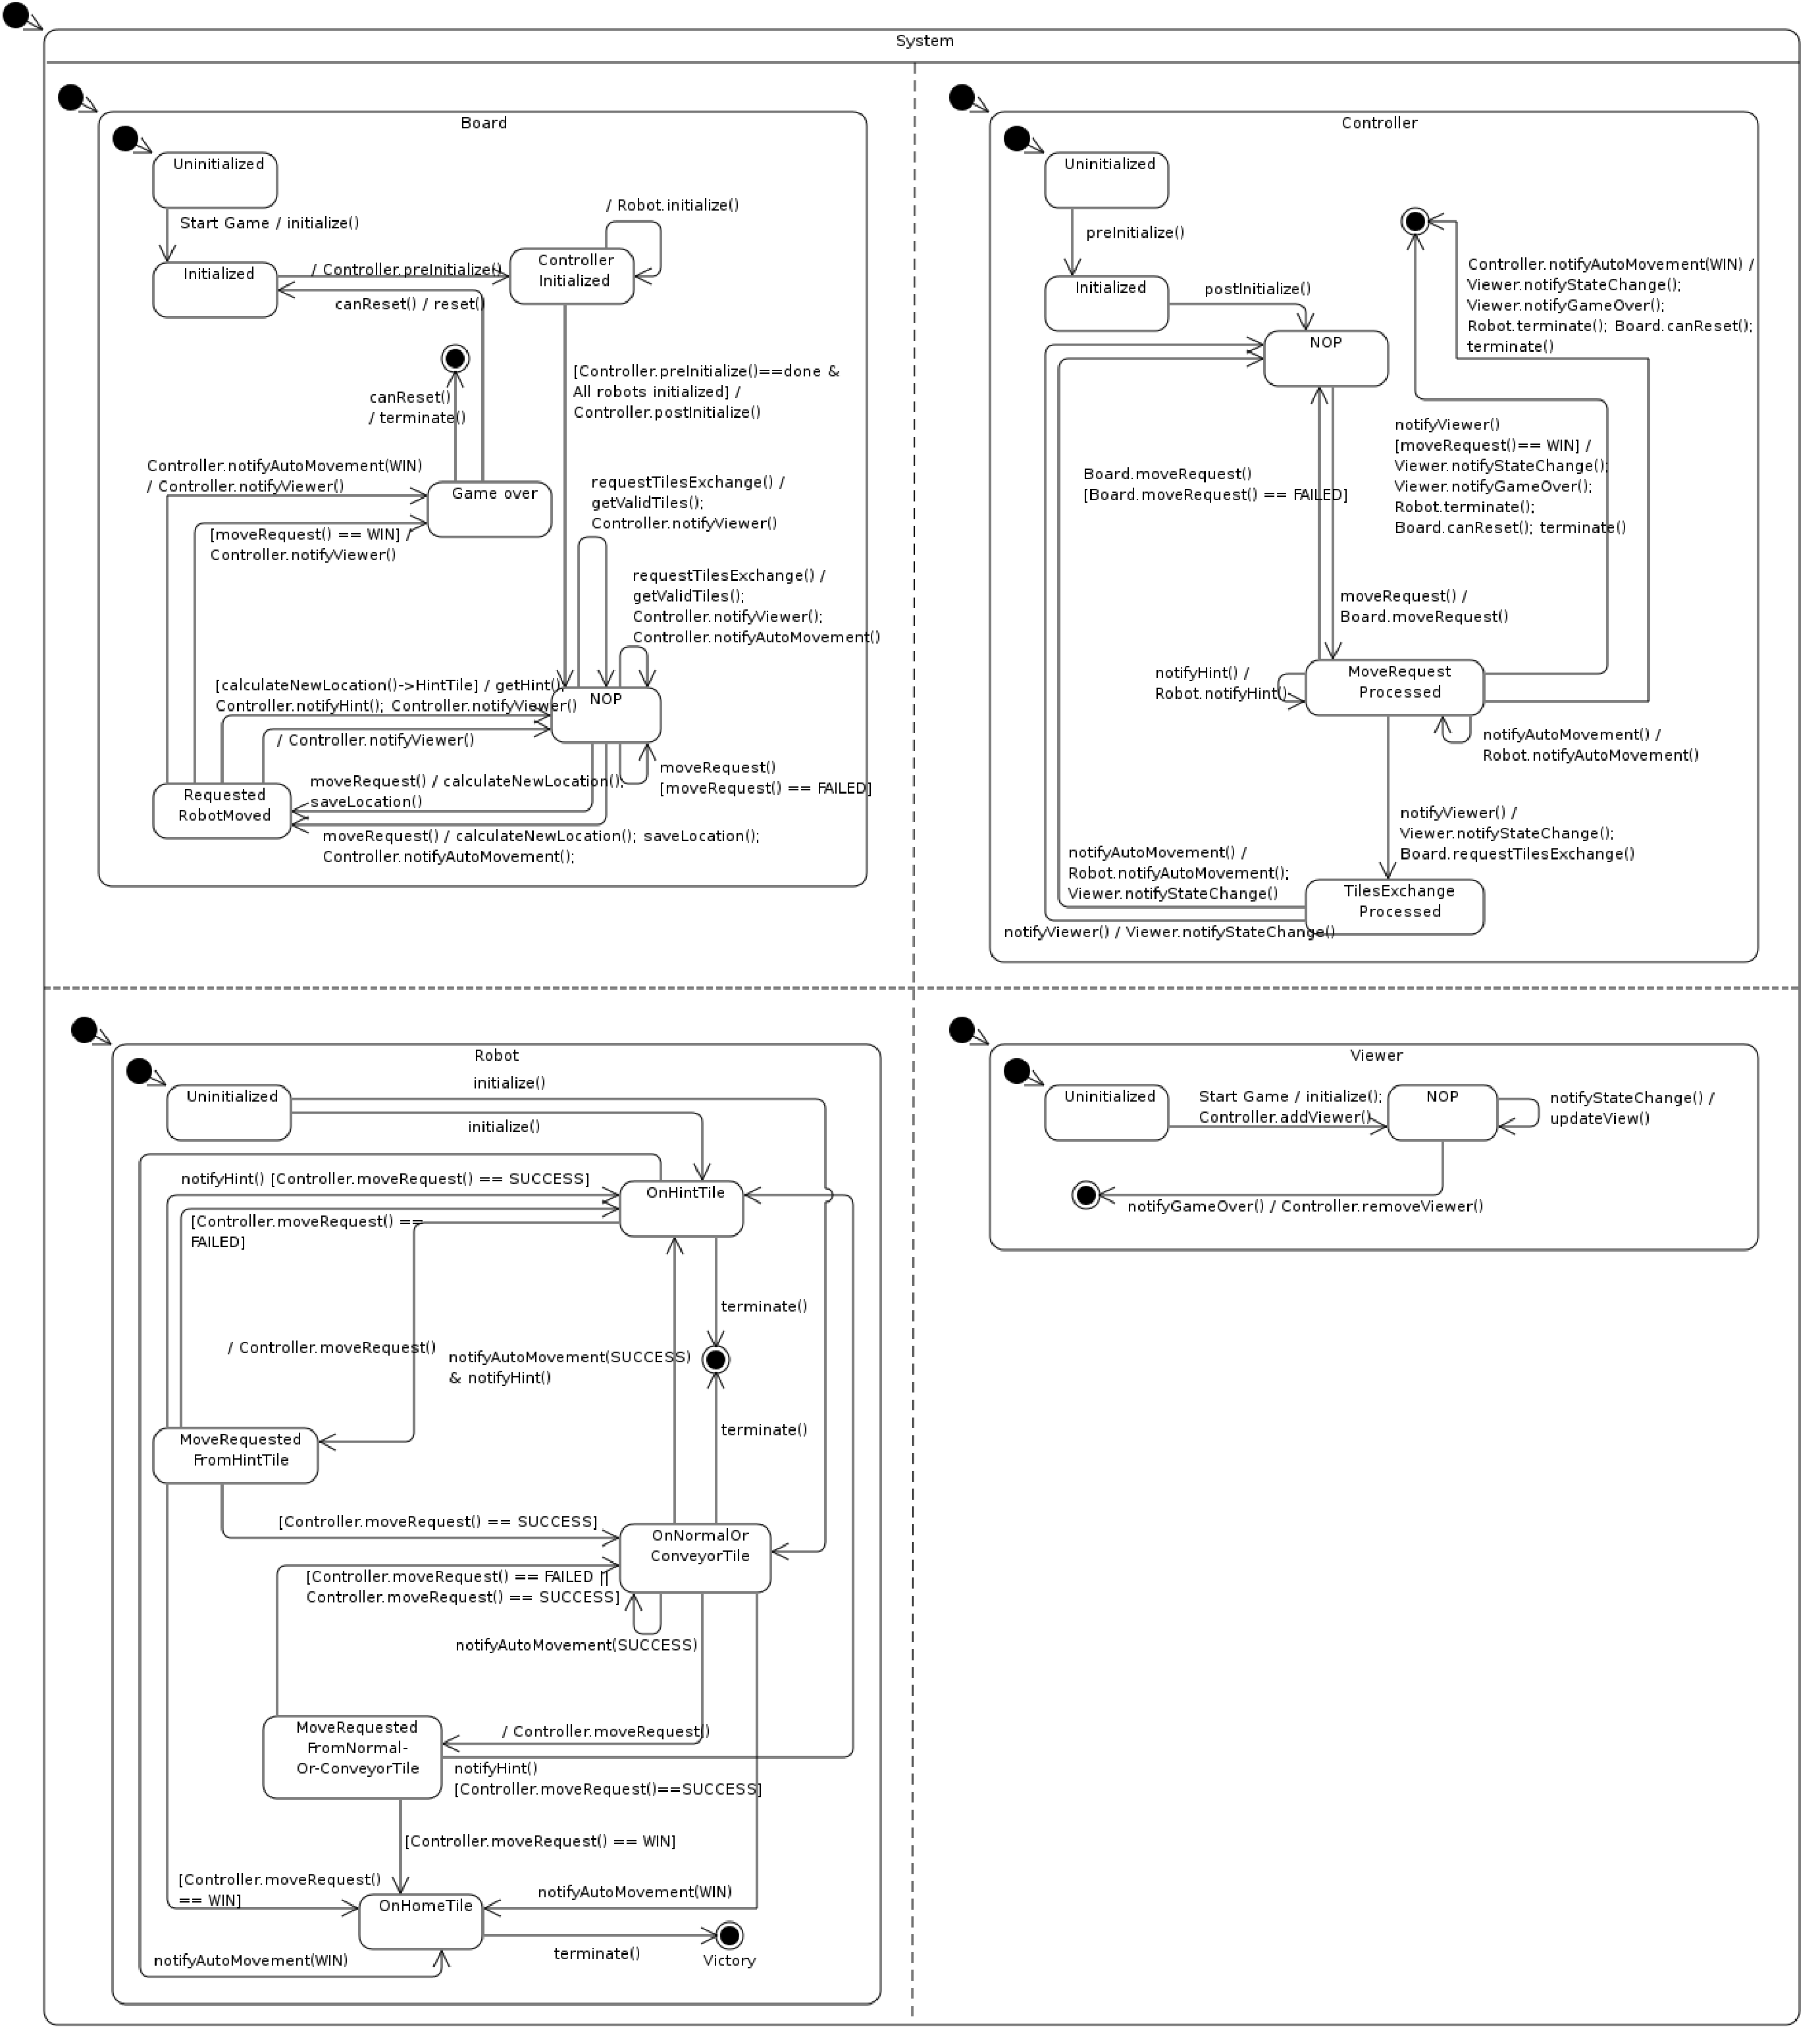
\includegraphics[width=\linewidth]{statecharts/system.pdf}
	
